\section{Основная часть}

\subsection{Анализ исторических прототипов и современных прототипов}
\subsubsection{Шахматы}
Первым прототипом современных шахмат считается индийская игра Чатуранга~\cite{web:wiki-chess-history}. В
последствии игра попала к персам под названием чатранг. После завоевания
арабами Персии первые познакомились с чатрангом; в арабском языке название игры
стало звучать как шатрандж.

Наибольшее изменение чатуранга претерпела, распространяясь на восток из
Индии,где в результате возникли несколько игр,сильно отличавшихся друг от
друга, и от современных шахмат. В Китае появилась игра сянци. В Таиланде
появилась игра Макрук. В Японии появилась игра Сёги (или Шоги).

В Европе современные шахматные правила начали возникать в XV --- XVII веках.
Приблизительно в 1475 году были совершенны два значительных изменения в
шахматах: ферзь, ранее перемещавшийся только на одно поле по диагонали, получил
возможность ходить на любое количество полей в любом направлении и стал
сильнейшей фигурой, а ''прыжок'' слона был заменён на перемещение по диагонали на
любое количество полей.

Шахматные правила окончательно сформировались в XVIII веке.\\
Игра происходит на доске, поделённой на равные квадратные клетки, или поля.
Размер доски — 8×8 клеток. Вертикальные ряды полей (вертикали) обозначаются
латинскими буквами от а до h слева направо, горизонтальные ряды (горизонтали) —
цифрами от 1 до 8 снизу вверх; каждое поле обозначается сочетанием
соответствующих буквы и цифры. Поля раскрашены в тёмный и светлый цвета (и
называются, соответственно, чёрными и белыми) так, что соседние по вертикали и
горизонтали поля раскрашены в разные цвета. Доска располагается так, чтобы
ближнее угловое поле справа от игрока было белым (для белых это поле h1, для
чёрных — поле а8).

У игроков в начале игры имеется по одинаковому набору фигур. Фигуры одного из
игроков условно называются «белыми», другого — «чёрными». Белые фигуры окрашены
в светлый цвет, чёрные — в тёмный. Сами игроки называются «белые» и «чёрные» по
цвету своих фигур.

В каждый комплект фигур входят: король, ферзь, две ладьи, два слона, два коня и
восемь пешек. В начальной позиции фигуры обеих сторон размещаются так, как
показано на диаграмме (смотреть рисунок~\ref{fig:chess-pos}). Белые занимают
первую и вторую горизонтали, чёрные — седьмую и восьмую. Пешки расположены на
второй и седьмой горизонталях соответственно. 

\begin{figure}[htpb]
    \centering
    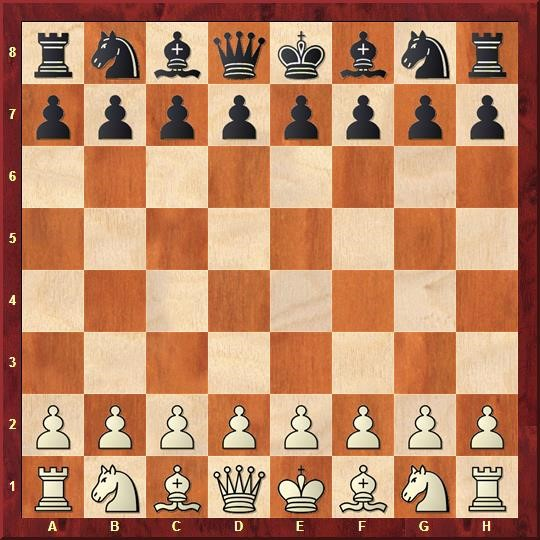
\includegraphics[width=0.8\textwidth]{chess-pos}
    \caption{Позиция шахматных фигур в начале игры}%
    \label{fig:chess-pos}
\end{figure}

Так же существует разновидность шахмат, специализированная для слабовидящих
людей. Хотя большинство правил в слепых шахматах соответствуют обычным
шахматам, есть несколько модификаций, чтобы помочь слепым и слабовидящим
игрокам (рис.~\ref{fig:blind-chess})~\cite{web:wiki-ibca}:
\begin{enumerate}
    \item Любой из игроков может потребовать использования двух досок: зрячий
        игрок использует обычную доску, а \gls{blind-man} использует доску,
        специально сконструированную следующим образом: 
        \begin{enumerate}
            \item Все чёрные квадраты возвышаются примерно на 3--4 мм над
                белыми. Нащупывая квадраты, игрок может определить, является ли
                квадрат чёрным или белым.
            \item Каждый из квадратов на доске имеет отверстие в центре, чтобы
                шахматные фигуры могли быть закреплены в этих отверстиях.
            \item Каждая фигура имеет в основании направленный вниз выступ
                (гвоздь), который входит в отверстия в квадратах на доске, тем
                самым надёжно фиксируясь на доске.
            \item На верхушках всех чёрных фигур закреплена булавка, помогающая
                игроку различать белую и чёрную фигуры.
        \end{enumerate}
\end{enumerate}
\begin{figure}[H]
    \centering
    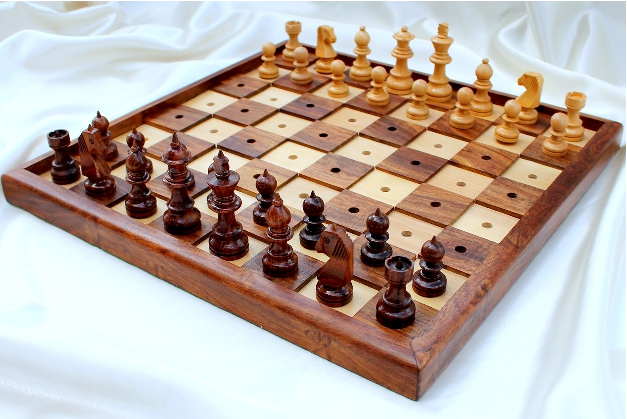
\includegraphics[width=0.9\textwidth]{blind-chess}
    \caption{Стандартизованные шахматы для слабовидящих людей}\label{fig:blind-chess}
\end{figure}

\subsubsection{Методы расширения аудитории}
На текущий момент главным средством расширения аудитории является
рекламирования изделия.

Одним из первых методов рекламирования своих товаров было использование
глашатаев. Он характеризовался малой скоростью распространения информации,
высокими ценовыми издержками и отсутствием определённой направленности
аудитории.

После изобретения книгопечатания и его распространения, стало возможно
выпускать периодические издания (газеты), в которых размещалась, помимо
новостей, реклама. Этот метод характеризовался более быстрой скоростью
распространения информации (но всё ещё не достаточно быстрой), значительно
более низкими ценовыми издержками (но они всё ещё напрямую зависят от охвата
аудитории), более узким охватом аудитории (только для людей, читающих на
постоянной основе газеты и журналы).

Следующей важной точкой в методах распространения информации, стало изобретение
телеграфа. Оно позволило моментально распространять ограниченное количество
информации на условно бесконечное расстояние. Характеризуется невероятно
высокой скоростью распространения информации, издержками, близкими к нулю,
охватом невероятно малой аудитории (1 человек) (можно исправить при
использовании газет).

Не менее важным моментом в истории распространения информации, по моему мнения,
является изобретение радио и телевидения. Оно связало между собой огромные
расстояния. Характеризуется так же, как и телеграфные сообщения, но не имеет
недостатка в виде узкой целенаправленности рекламирования.

Революцию в распространении информации произвело появление в 29 октября 1969
года интернета\gls{chess-not}и последующее его распространение. Сейчас это самый большой
централизованный метод передачи информации и рекламирования товаров или услуг.
Характеризуется моментальной передачей информации, независимо от расстояния,
практически отсутствием издержек, охватом огромной аудитории (каждый человек,
пользующийся интернетом). В настоящее время это лучший метод рекламирования.

\subsection{Теоретическая часть}
\subsubsection{Тактильные шахматы}
В процессе анализа были сформированы следующие минимально необходимые критерии
для будущего изделия:
\begin{enumerate}
    \item возможность быстро ощупать большое число фигур;
    \item сложность случайно сдвинуть или уронить фигуру;
    \item возможность легко и быстро нащупать границы поля на доске;
    \item удобство во время игры;
    \item удобство при складывании и раскладывании фигур и доски;
    \item простота и низкая стоимость изготовления.
\end{enumerate}
Для осуществления первого критерия я решил использовать идеи восточноазиатских
аналогов европейских шахмат. В сянци и сёги фигуры представляют собой не резные
статуэтки, а плоские таблички: в форме пятиугольника и в форме круга
соответственно (рис.~\ref{fig:shogi},~\ref{fig:syanci}). Использование такой
формы позволит слепому шахматисту не бояться зацепиться за какую-либо другую
фигуру при движении рукой и ощупывании фигур. Так же это усовершенствование
позволит значительно упростить производства фигурок и сделать его дешевле, что
влияет на шестой пункт выше перечисленных критериев.
\begin{figure}[h]
    \begin{minipage}[h]{0.5\linewidth}
        \center{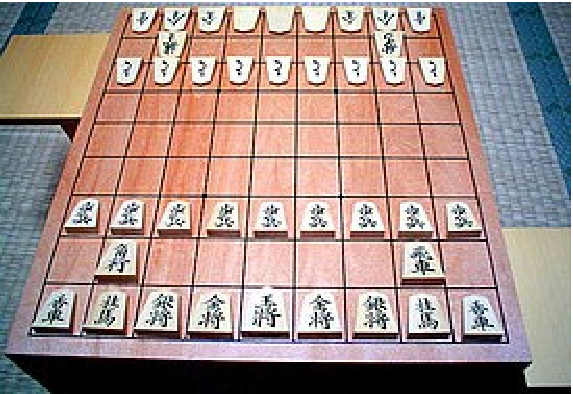
\includegraphics[width=0.9\linewidth]{shogi}}
        \caption{Сёги}\label{fig:shogi}
    \end{minipage}
    \begin{minipage}[h]{0.5\linewidth}
        \center{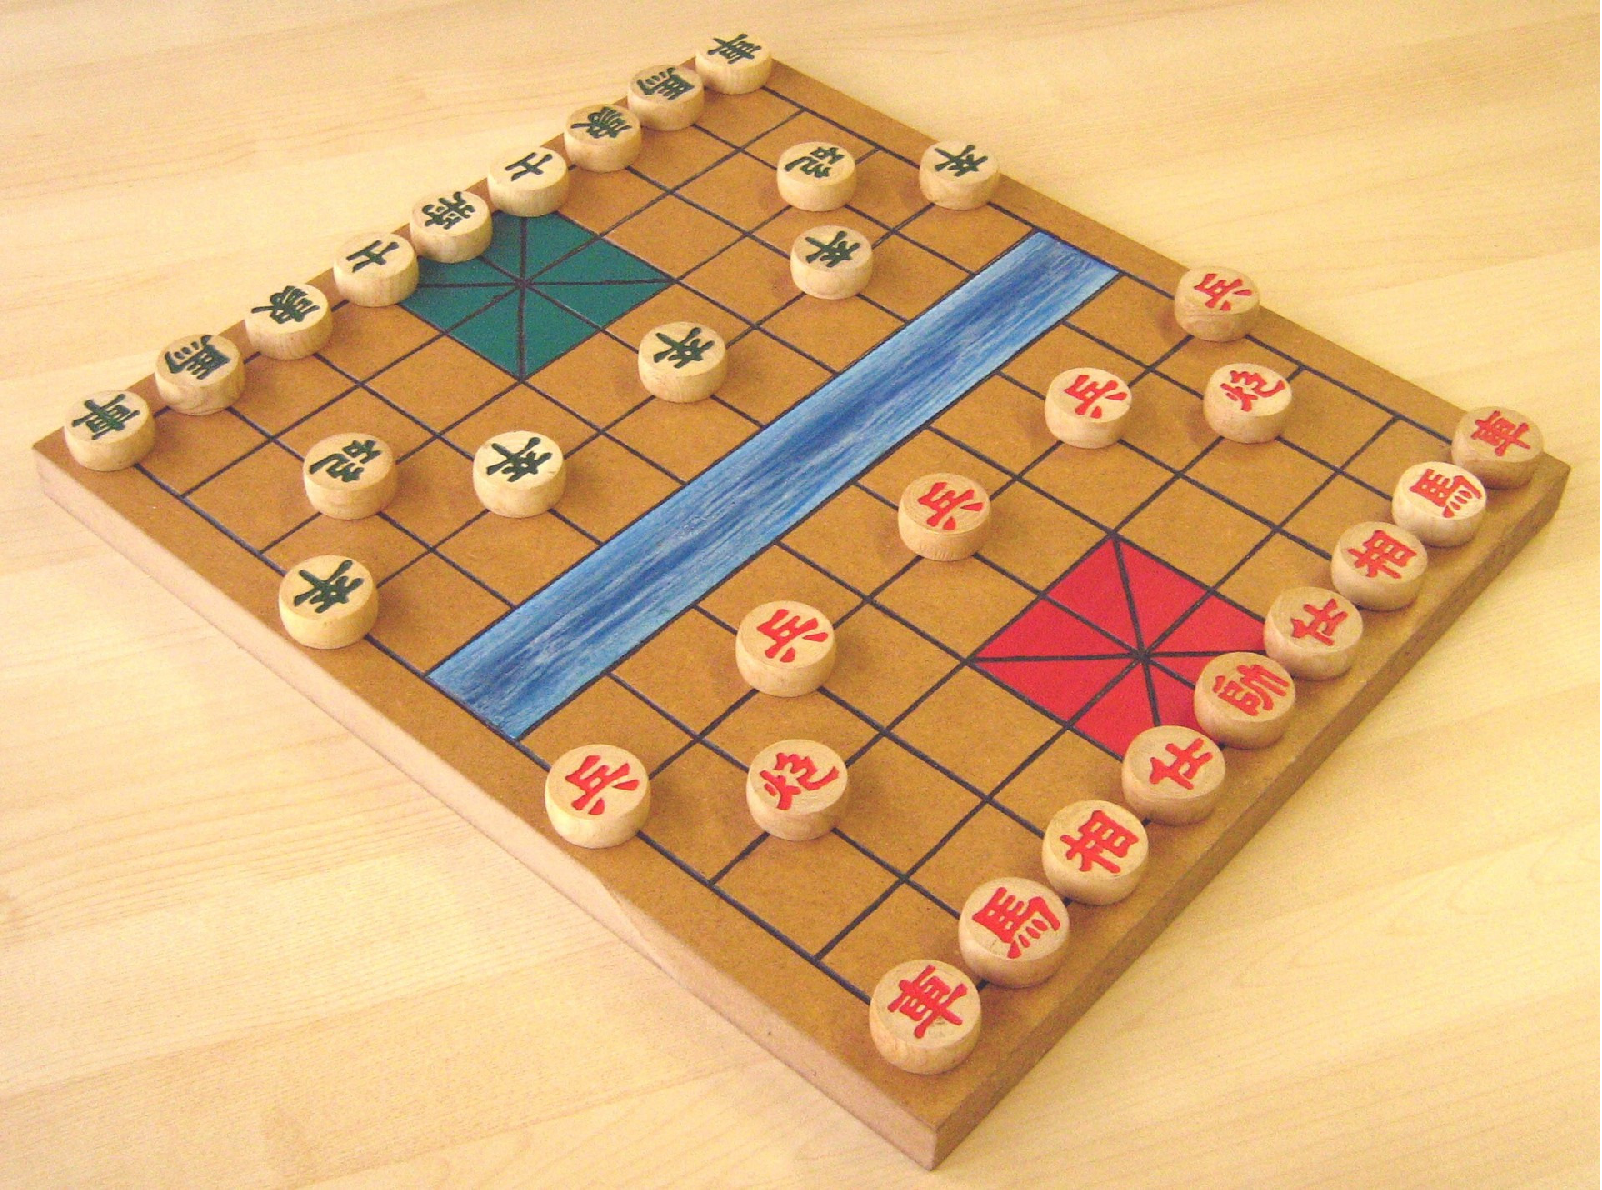
\includegraphics[width=0.9\linewidth]{syanci}}
        \caption{Сянци}\label{fig:syanci}
    \end{minipage}
\end{figure}

В официальных стандартизированных шахматах во избежание случайного падения
фигуры по вине одного из игроков используются специальные фигуры, имеющие
небольшой штырь внизу фигуры, который вставляется при ходе в отверстия,
имеющиеся в центре каждого из полей на шахматной доске
(рис.~\ref{fig:blind-chess}). Для упрощения изготовление мною было принять
решение избавиться от штыря под фигурой и, вместо небольших отверстий, вырезать
углубления, диаметр которых будет равен диаметру фигур.
\begin{figure}[h]
    \centering
    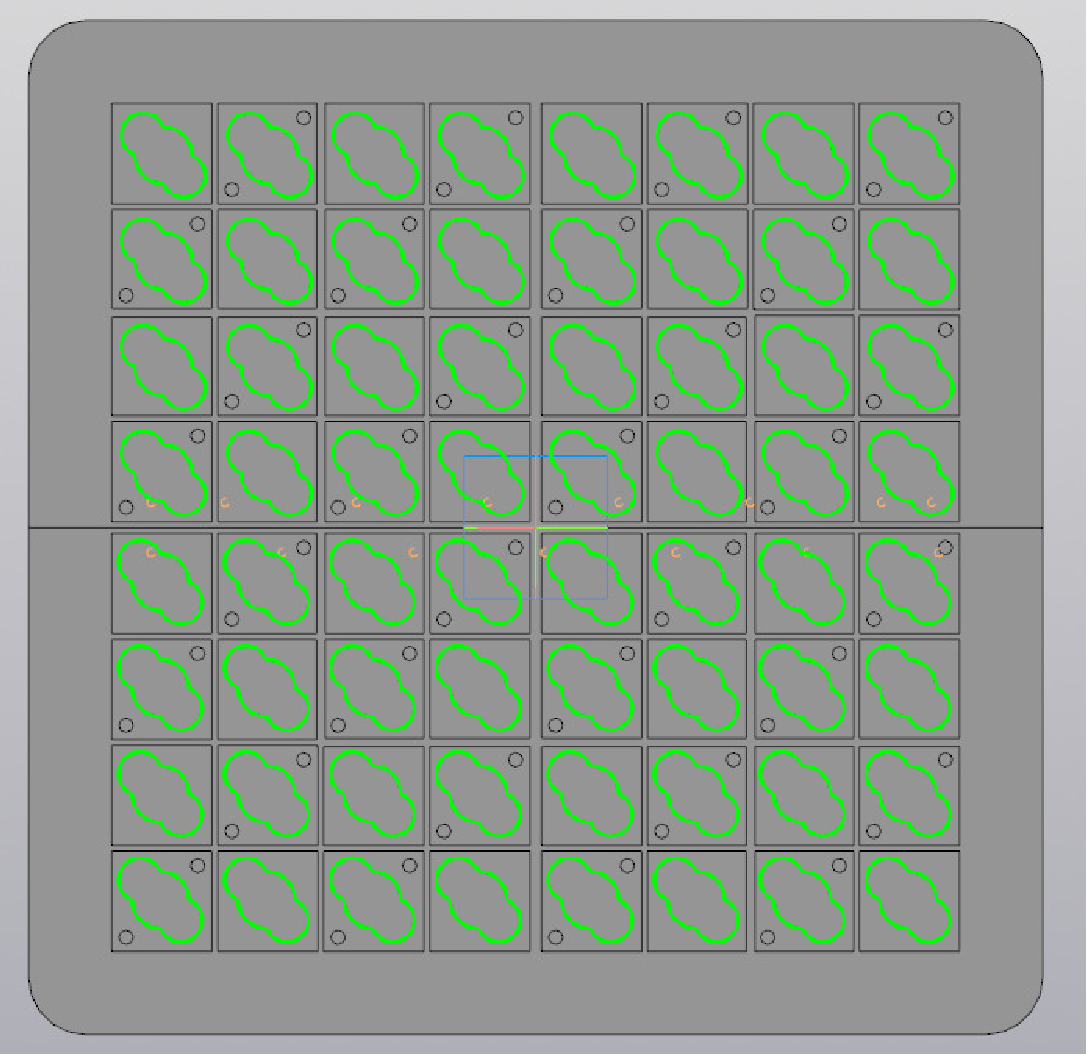
\includegraphics[width=0.8\textwidth]{shtir}
    \caption{Углубления в доске}\label{fig:shtir}
\end{figure}

Для снижения стоимости и упрощения изготовления шахмат мною было решено отказаться от
разницы в уровнях между чёрными и белыми клетками. Вместо этого предполагалось
использовать квадратную сетку, накладывающуюся на доску при изготовлении. Так
же для упрощения ориентации на игровом поле было решено сделать толщину прутьев
не равномерной: для центральных линий (горизонтальной и вертикальной) было
сделано двойное утолщение, а для центральных линий в каждом секторе, которые
были образованы выше указанными центральными линиями, было сделано полуторное
утолщение.

Для упрощения складывания и раскладывания фигур на шахматном поле, мною так же
было решено отказаться от полости внутри шахмат, обычно используемой в шахматах
массового производства. Вместо неё в днище был предусмотрен набор симметричных
относительно линии сгиба и перпендикулярной её линии отверстий. Он позволит не
перемешиваться фигуркам и будет удобнее брать их. Так же, при условии
систематического складывания фигур, это очень упростит начало новой партии,
уменьшив время, необходимое для раскладывания фигур.

Во избежание путаницы во время игры в шахматы, было решено отказаться от шрифта
Брайля, которая могла возникнуть из-за перевёрнутости фигур противника
относительно игрока, что могло привести к не правильному чтению названия
фигурок. За место него была выбрана английская \gls{chess-not}. Она позволяет
назвать любую шахматную фигуру по шаблону <Цвет><Название> используя
минимальное число букв, а так же она достаточно распространена в мире. Русская
\gls{chess-not} не удовлетворяла меня тем, что фигура короля обозначается в ней как
''Кр'', то есть использует больше букв, чем в английской нотации.

Для универсальности было принято решение интегрировать в шахматный набор шашки.
Для этого фигуры были сделаны двухсторонним: с одной стороны на фигуре была
шахматная нотация, а на другой стороне была шашечная нотация.

\subsubsection{Реклама}
При анализе возможных платформ рекламирования изделия, мною была выбрана
интернет--площадка, так как это быстро развивающаяся популярная платформа не
только для рекламирования изделий, но и для последующей продажи изделия. Даже
не смотря на то, что ею пользуются исключительно люди без проблем со зрением,
через этих людей узнают те, у кого есть проблемы со зрением. Благодаря этому,
получится охватить гораздо большую аудиторию, чем при аудио--рекламе, которая
хорошо воспринимается слабовидящими людьми.

\subsection{Практическая часть}
\subsubsection{Создание тактильных шахмат}
При анализе возможных методов изготовления, была выбрана модель ``слоёного
пирога'', так как она проста в своём изготовлении и требует менее сложное и
дорогостоящее оборудование. Для такого метода изготовления, по моему мнению,
идеально подойдёт фанера, так как она дешёвая, легкодоступная, экологичная и её
легко обрабатывать. В качестве технологи вырезания элементов доски из фанеры,
мною была выбрана технология лазерного прожигания фанеры. С этой целью мною был
использован лазерный гравер RUKA 6040XY Бизнес.

Для накладных элементов (буквы на фигурах, буквы и цифры на краях доски) было
решено не использовать фанеру, так как если вырезать буквы на этих элементах,
то они будут плохо читаемые, а если вырезать из них буквы и в последствии
поочерёдно наклеивать на доску, то будут проблемы с выравниванием их
относительно друг друга и относительно доски. Фанера была заменена на
пластмассу для печати на 3D--принтере, так как использование технологи
3D--печати позволяет полностью автоматизировать процесс изготовления накладных
элементов. С этой целью мною был использован 3D--принтер Anet A8.

Для склеивания слоёв фанеры между собою, был использован клей ПВА,
специализированный для склеивания древесины. Для обработки готового изделию был
использован лак. 

\subsubsection{Разработка рекламы}
Для создания рекламного баннера был выбран визуальный редактор \gls{inkscape},
так как он реализует векторную графику, обладает широким функционалом и распространяется по открытой
лицензии.

Для рекламы на интернет--площадках, мною была выбрана форма
\gls{banner}а~\cite{web:wiki-banner}. Она предполагает прямоугольную форму с
соотношением сторон 1 к 2. Стандартным разрешением (соотношением высоты
изображения к его ширине) для рекламного \gls{banner}а используется
320\acrshort{px} на 640\acrshort{px}. Используя \gls{gold-ratio} для построения
общего макета баннера, получим рисунок~\ref{fig:base-template}. Чёрными
точками и утолщёнными линиями отмечены места, где должны располагаться наиболее
значимые элементы рекламы (например, название изделия, изображение изделия,
товарный знак). Разместив все необходимые элементы, получим следующий макет
рекламы (смотреть рисунок~\ref{fig:adversting-template}). Разместив текст в
поля, размеченные на рисунке~\ref{fig:adversting-template}, получим финальное
изображение макета (смотреть рисунок~\ref{fig:adversting-final}). После
добавления \gls{gradient}ного заднего фона, получаем финальное изображение рекламного
\gls{banner}а (смотреть рисунок~\ref{fig:adv-final}).
\begin{figure}[htpb]
    \begin{center}
        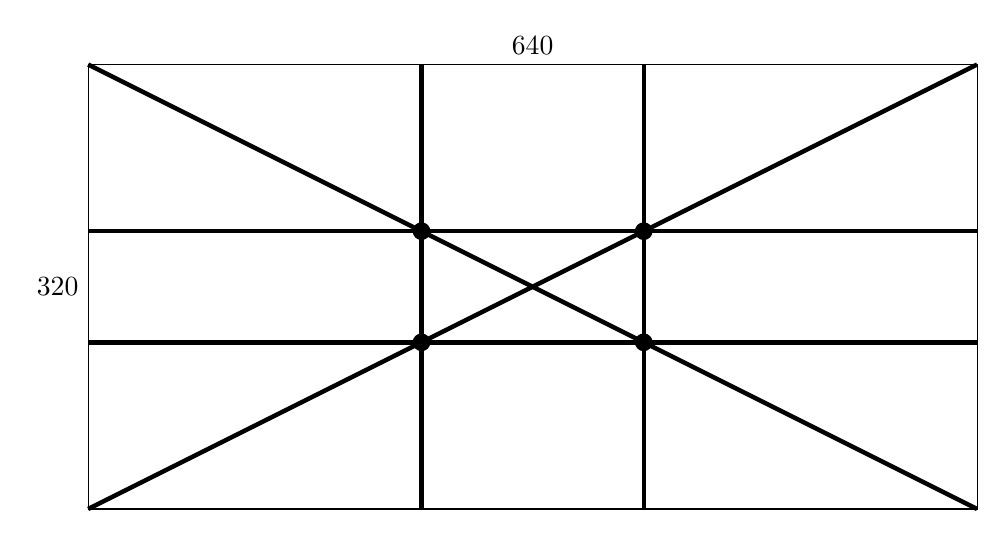
\begin{tikzpicture}[scale=0.5]
            \coordinate (A) at (-320px,-160px);
            \coordinate (B) at (-320px,160px);
            \coordinate (C) at (320px,160px);
            \coordinate (D) at (320px,-160px);

            \draw (A)
                -- node[left] {320} (B)
                -- node[above] {640} (C)
                -- (D)
                -- cycle;

            \draw[ultra thick] (A) -- (C);
            \draw[ultra thick] (B) -- (D);

            \draw[ultra thick] (-320px,{160px*0.250}) -- +(640px,0);
            \draw[ultra thick] (-320px,-{160px*0.250}) -- +(640px,0);
            \draw[ultra thick] (-{320px*0.250},-160px) -- +(0,320px);
            \draw[ultra thick] ({320px*0.250},-160px) -- +(0,320px);

            \draw[fill=black] (-{320px*0.250},-{160px*0.250}) circle (6pt);
            \draw[fill=black] (-{320px*0.250},{160px*0.250}) circle (6pt);
            \draw[fill=black] ({320px*0.250},{160px*0.250}) circle (6pt);
            \draw[fill=black] ({320px*0.250},-{160px*0.250}) circle (6pt);
        \end{tikzpicture}
    \end{center}
    \caption{Макет рекламного баннера}%
    \label{fig:base-template}
\end{figure}

\begin{figure}[H]
    \centering
    
\includegraphics[width=0.8\textwidth]{adversting}
    \caption{Макет рекламного \gls{banner}а с разметкой полей}\label{fig:adversting-template}
\end{figure}

\begin{figure}[htpb]
    \centering
    
\includegraphics[width=0.8\textwidth]{adversting-final}
    \caption{Конечный шаблон рекламы}\label{fig:adversting-final}
\end{figure}

\begin{figure}[htpb]
    \centering
    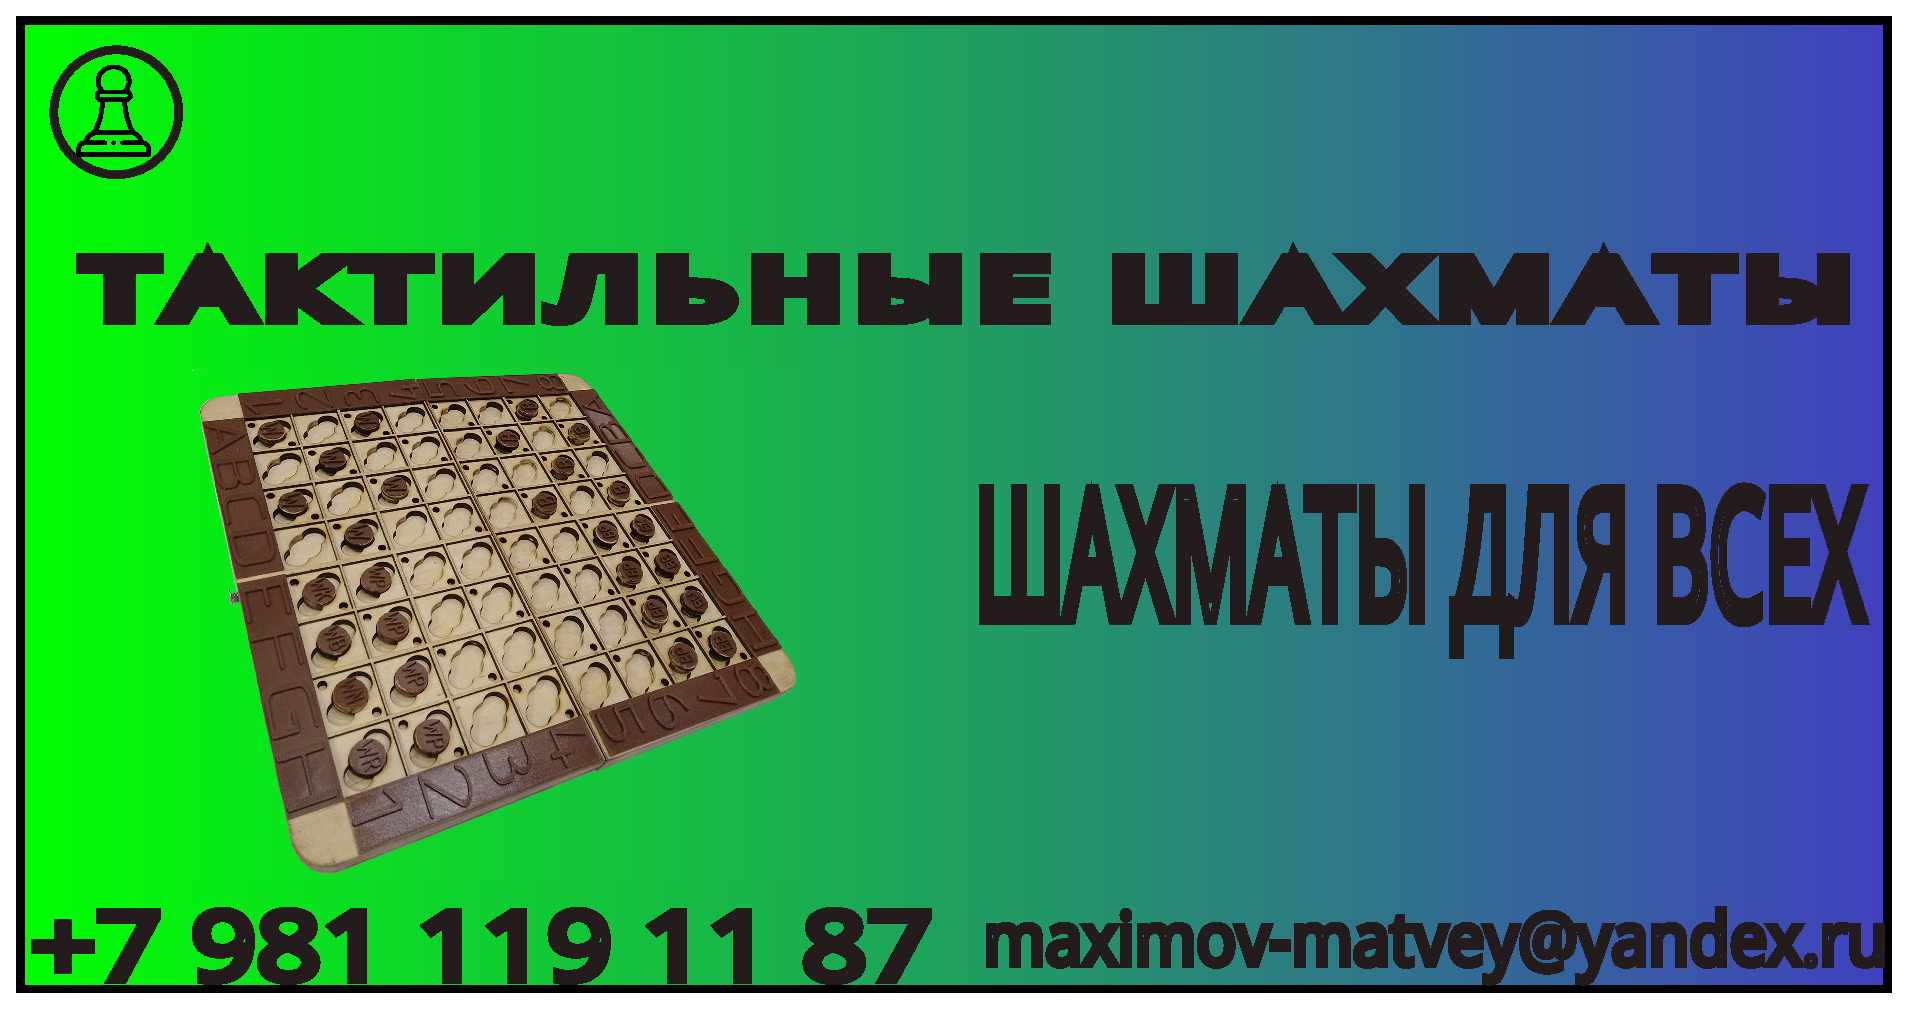
\includegraphics[width=0.8\textwidth]{adv-final.eps}
    \caption{Финальное изображение рекламного баннера}%
    \label{fig:adv-final}
\end{figure}
